
%%%%%%%%%%%%%%%%%%%%%%%%%%%%%%%%%%%%%%%%%%%%%%%%%%%%%%%%%%%%%%%%%%%%%%%%%%%%%%%

\documentclass[12pt, a4paper, oneside]{article} 

%%%%%%%%%%%%%%%%%%%%%%%%%%%%%%%%%%%%%%%%%%%%%%%%%%%%%%%%%%%%%%%%%%%%%%%%%%%%%%%

\usepackage[brazilian]{babel} %% Portuguese words (capítulo, seção, etc.)
\usepackage[utf8]{inputenc} %% Suport to utf8 characthers

%% Math symbols, fonts and text
\usepackage{amsfonts, amsmath, amstext, amsthm, amssymb} 

\usepackage{color, xcolor} %% Colors packages
\definecolor{c1}{rgb}{0,0,1} % blue
\definecolor{c2}{rgb}{0,0.3,0.9} % light blue
\definecolor{c3}{rgb}{0.3,0,0.9} % red blue

\usepackage[colorlinks=true,breaklinks,brazilian]{hyperref} 
\hypersetup{
    linkcolor={c1}, % internal links
    citecolor={c2}, % citations
    urlcolor={c3}   % external links/urls
}

\usepackage{blindtext} %% Used to create dummy text (usefull for formating)

\usepackage[top=3cm,bottom=2cm,left=2.5cm,right=2.5cm]{geometry}

\usepackage{graphicx}  %% Used to insert images

%%%%%%%%%%%%%%%%%%%%%%%%%%%%%%%%%%%%%%%%%%%%%%%%%%%%%%%%%%%%%%%%%%%%%%%%%%%%%%%

%% Formating commands

\newcommand{\nl}{\newline}
\newcommand{\jump}{\nl\nl}
\newcommand{\paren}[1]{\left( #1 \right)}
\newcommand{\bracket}[1]{\left\{ #1 \right\}}
\newcommand{\sqrtbracket}[1]{\left[ #1 \right]}
\newcommand{\angbracket}[1]{\left\langle #1 \right\rangle}
\newcommand{\ceil}[1]{\left\lceil #1 \right\rceil}
\newcommand{\floor}[1]{\left\lfloor #1 \right\rfloor}

%%% Symbols

\newcommand{\pinf}{+\infty}
\newcommand{\minf}{-\infty}

%% Math commands

\newcommand{\abs}[1]{\left| #1 \right|}
\newcommand{\dlim}{\displaystyle\lim}
\newcommand{\dsum}{\displaystyle\sum}
\newcommand{\dprod}{\displaystyle\prod}
\newcommand{\dint}{\displaystyle\int}
\newcommand{\deriv}[1]{\dfrac{d}{d#1}}
\newcommand{\inv}{^{-1}}
\newcommand{\pow}[2]{#1^{#2}}
\newcommand{\sub}[2]{#1_{#2}}
\newcommand{\powsub}[3]{#1^{#2}_{#3}}
\newcommand{\subpow}[3]{#1^{#3}_{#2}}
\newcommand{\psint}[2]{\powsub{\dint}{#1}{#2}}
\newcommand{\spint}[2]{\subpow{\dint}{#1}{#2}}
\newcommand{\pssum}[2]{\powsub{\dsum}{#1}{#2}}
\newcommand{\spsum}[2]{\subpow{\dsum}{#1}{#2}}
\newcommand{\psprod}[2]{\powsub{\dprod}{#1}{#2}}
\newcommand{\spprod}[2]{\subpow{\dprod}{#1}{#2}}
\newcommand{\serie}[2][n]{\subpow{\dsum}{#1 = #2}{\pinf}}
\newcommand{\slim}[2][x]{\sub{\dlim}{#1 \to #2}}

%%% Set commands

\newcommand{\set}[1]{\bracket{\ #1\ }}
\newcommand{\st}{\ | \ }

\newcommand{\R}{\mathbb{R}}
\newcommand{\Z}{\mathbb{Z}}
\newcommand{\Q}{\mathbb{Q}}
\newcommand{\N}{\mathbb{N}}
\newcommand{\C}{\mathbb{C}}
\newcommand{\I}{\mathbb{I}}
\newcommand{\myin}[1]{\in #1}
\newcommand{\inR}{\myin{\R}}
\newcommand{\inZ}{\myin{\Z}}
\newcommand{\inQ}{\myin{\Q}}
\newcommand{\inN}{\myin{\N}}
\newcommand{\inC}{\myin{\C}}
\newcommand{\inI}{\myin{\I}}


%%% Theorems environments

\theoremstyle{definition}
\newtheorem{defi}{Definição}

\theoremstyle{plain}
\newtheorem{teo}{Teorema}

\theoremstyle{definition}
\newtheorem*{dem}{Demonstração}

\theoremstyle{plain}
\newtheorem{lema}[teo]{Lema}

\theoremstyle{plain}
\newtheorem{corol}{Corolário}

\theoremstyle{definition}
\newtheorem*{obs}{Observação}

\theoremstyle{definition}
\newtheorem*{exemplo}{Exemplo}

\theoremstyle{definition}
\newtheorem*{exercicio}{Exercício}

\theoremstyle{plain}
\newtheorem*{problema}{Problema}

\theoremstyle{definition}
\newtheorem*{nota}{Notação}

\theoremstyle{definition}
\newtheorem{metodo}{Método}

%% Misc

\newcommand{\inner}[2]{\angbracket{\ #1 \ , \ #2 \ }}

\newcommand{\cqd}{\ \blacksquare} 

\title{Relatório - EP1}
\date{\today}
\author{Lucas Paiolla Forastiere}

%%%%%%%%%%%%%%%%%%%%%%%%%%%%%%%%%%%%%%%%%%%%%%%%%%%%%%%%%%%%%%%%%%%%%%%%%%%%%%%

\begin{document}

\maketitle

%%%%%%%%%%%%%%%%%%%%%%%%%%%%%%%%%%%%%%%%%%%%%%%%%%%%%%%%%%%%%%%%%%%%%%%%%%%%%%%
%%%%%%%%%%%%%%%%%%%%%%%%%%%%%%%%%%%%%%%%%%%%%%%%%%%%%%%%%%%%%%%%%%%%%%%%%%%%%%%

\section{Parte 1}

Utilizei apenas uma função, que é a mesma utilizada no Método de Newton.
Com ela tenho garantia que convergerá dentro de um intervalo dentrado
nas raízes. 

Como critérios de parada utilizei ou quando o valor absoluto de $f(x)$
aumenta de uma iteração para a outra (e daí concluímos que o método divergiu)
ou quando o valor absoluto de $f(x)$ fica menor que $EPS=10^{-12}$

Como resultados obtive:
\begin{enumerate}
    \item Pontos aproximadamente de $0$ para menor convergem 
    para $-0.539835$;
    \item Pontos entre $0.4$ e $0.6$ aproximadamente convergem para 
    $2.617867$;
    \item Pontos entre $0.67$ e $0.68$ aproximadamente convergem para
    $-0.539835$;
    \item O ponto $0.69$ converge novamente para $2.617867$;
    \item De $0.7$ até $2$, converge para $1.487962$;
    \item O ponto $2.1$ converge para  $-0.539835$;
    \item De aí para frente começa a convergir para $2.617867$;
    \item Apenas lá a partir de $710$ que começa a divergir;
    \item Já por pontos negativos, nem chegou a divergir.
\end{enumerate}

\section{Parte 2}

Na segunda parte, fiz vários testes. Os plots ficara muito bonitos, mas não consegui
achar aqueles pontinhos de divergência igual à foto do professor.

Podemos perceber que ao mudar uma constante, a imagem fica rotacionada.

Como critério de parada, utilizei uma função para igualdade de complexos
que considera as componentes reais e imaginárias (se ambas estão próximas
de zero).

As imagens geradas são mostradas a seguir:

\begin{figure}
    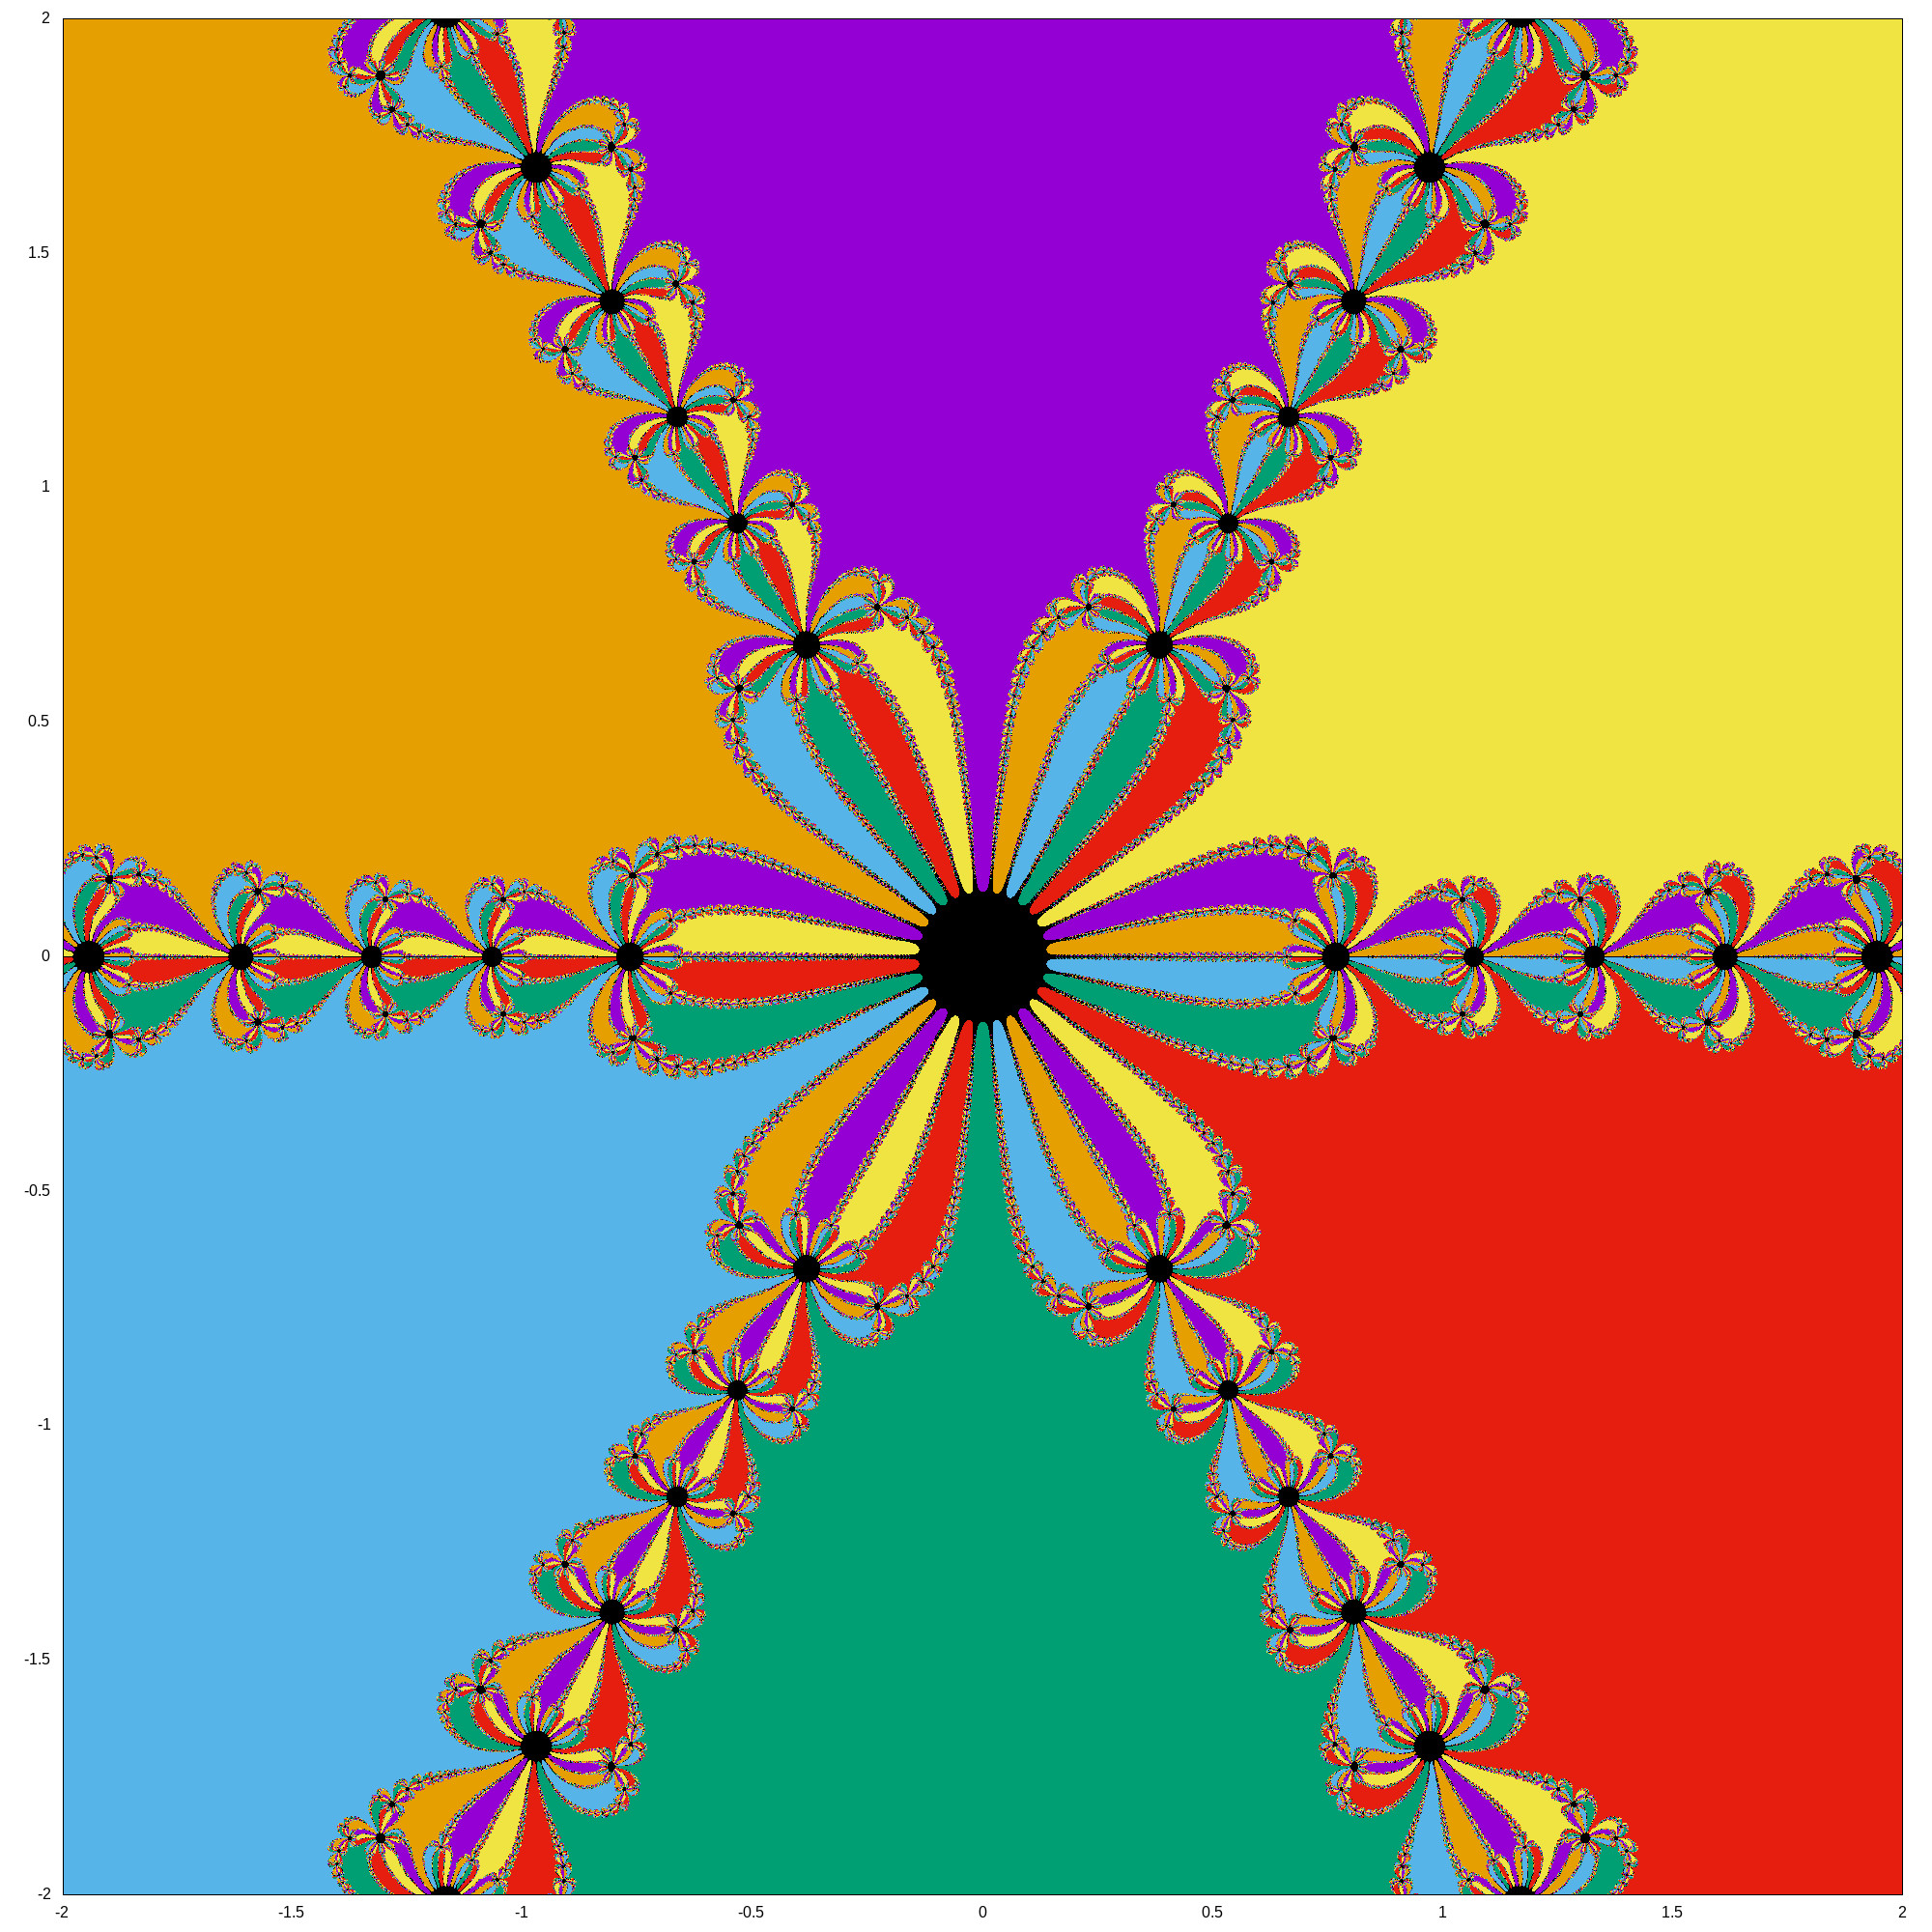
\includegraphics[width=\linewidth]{/home/giatro/Desktop/IME/3_Semestre/Laboratorio_de_Metodos_Numericos_MAC0210/EPs/1EP/f1.jpeg}
    \caption{$f_1(x)=x^6+1$}
\end{figure}

\begin{figure}
    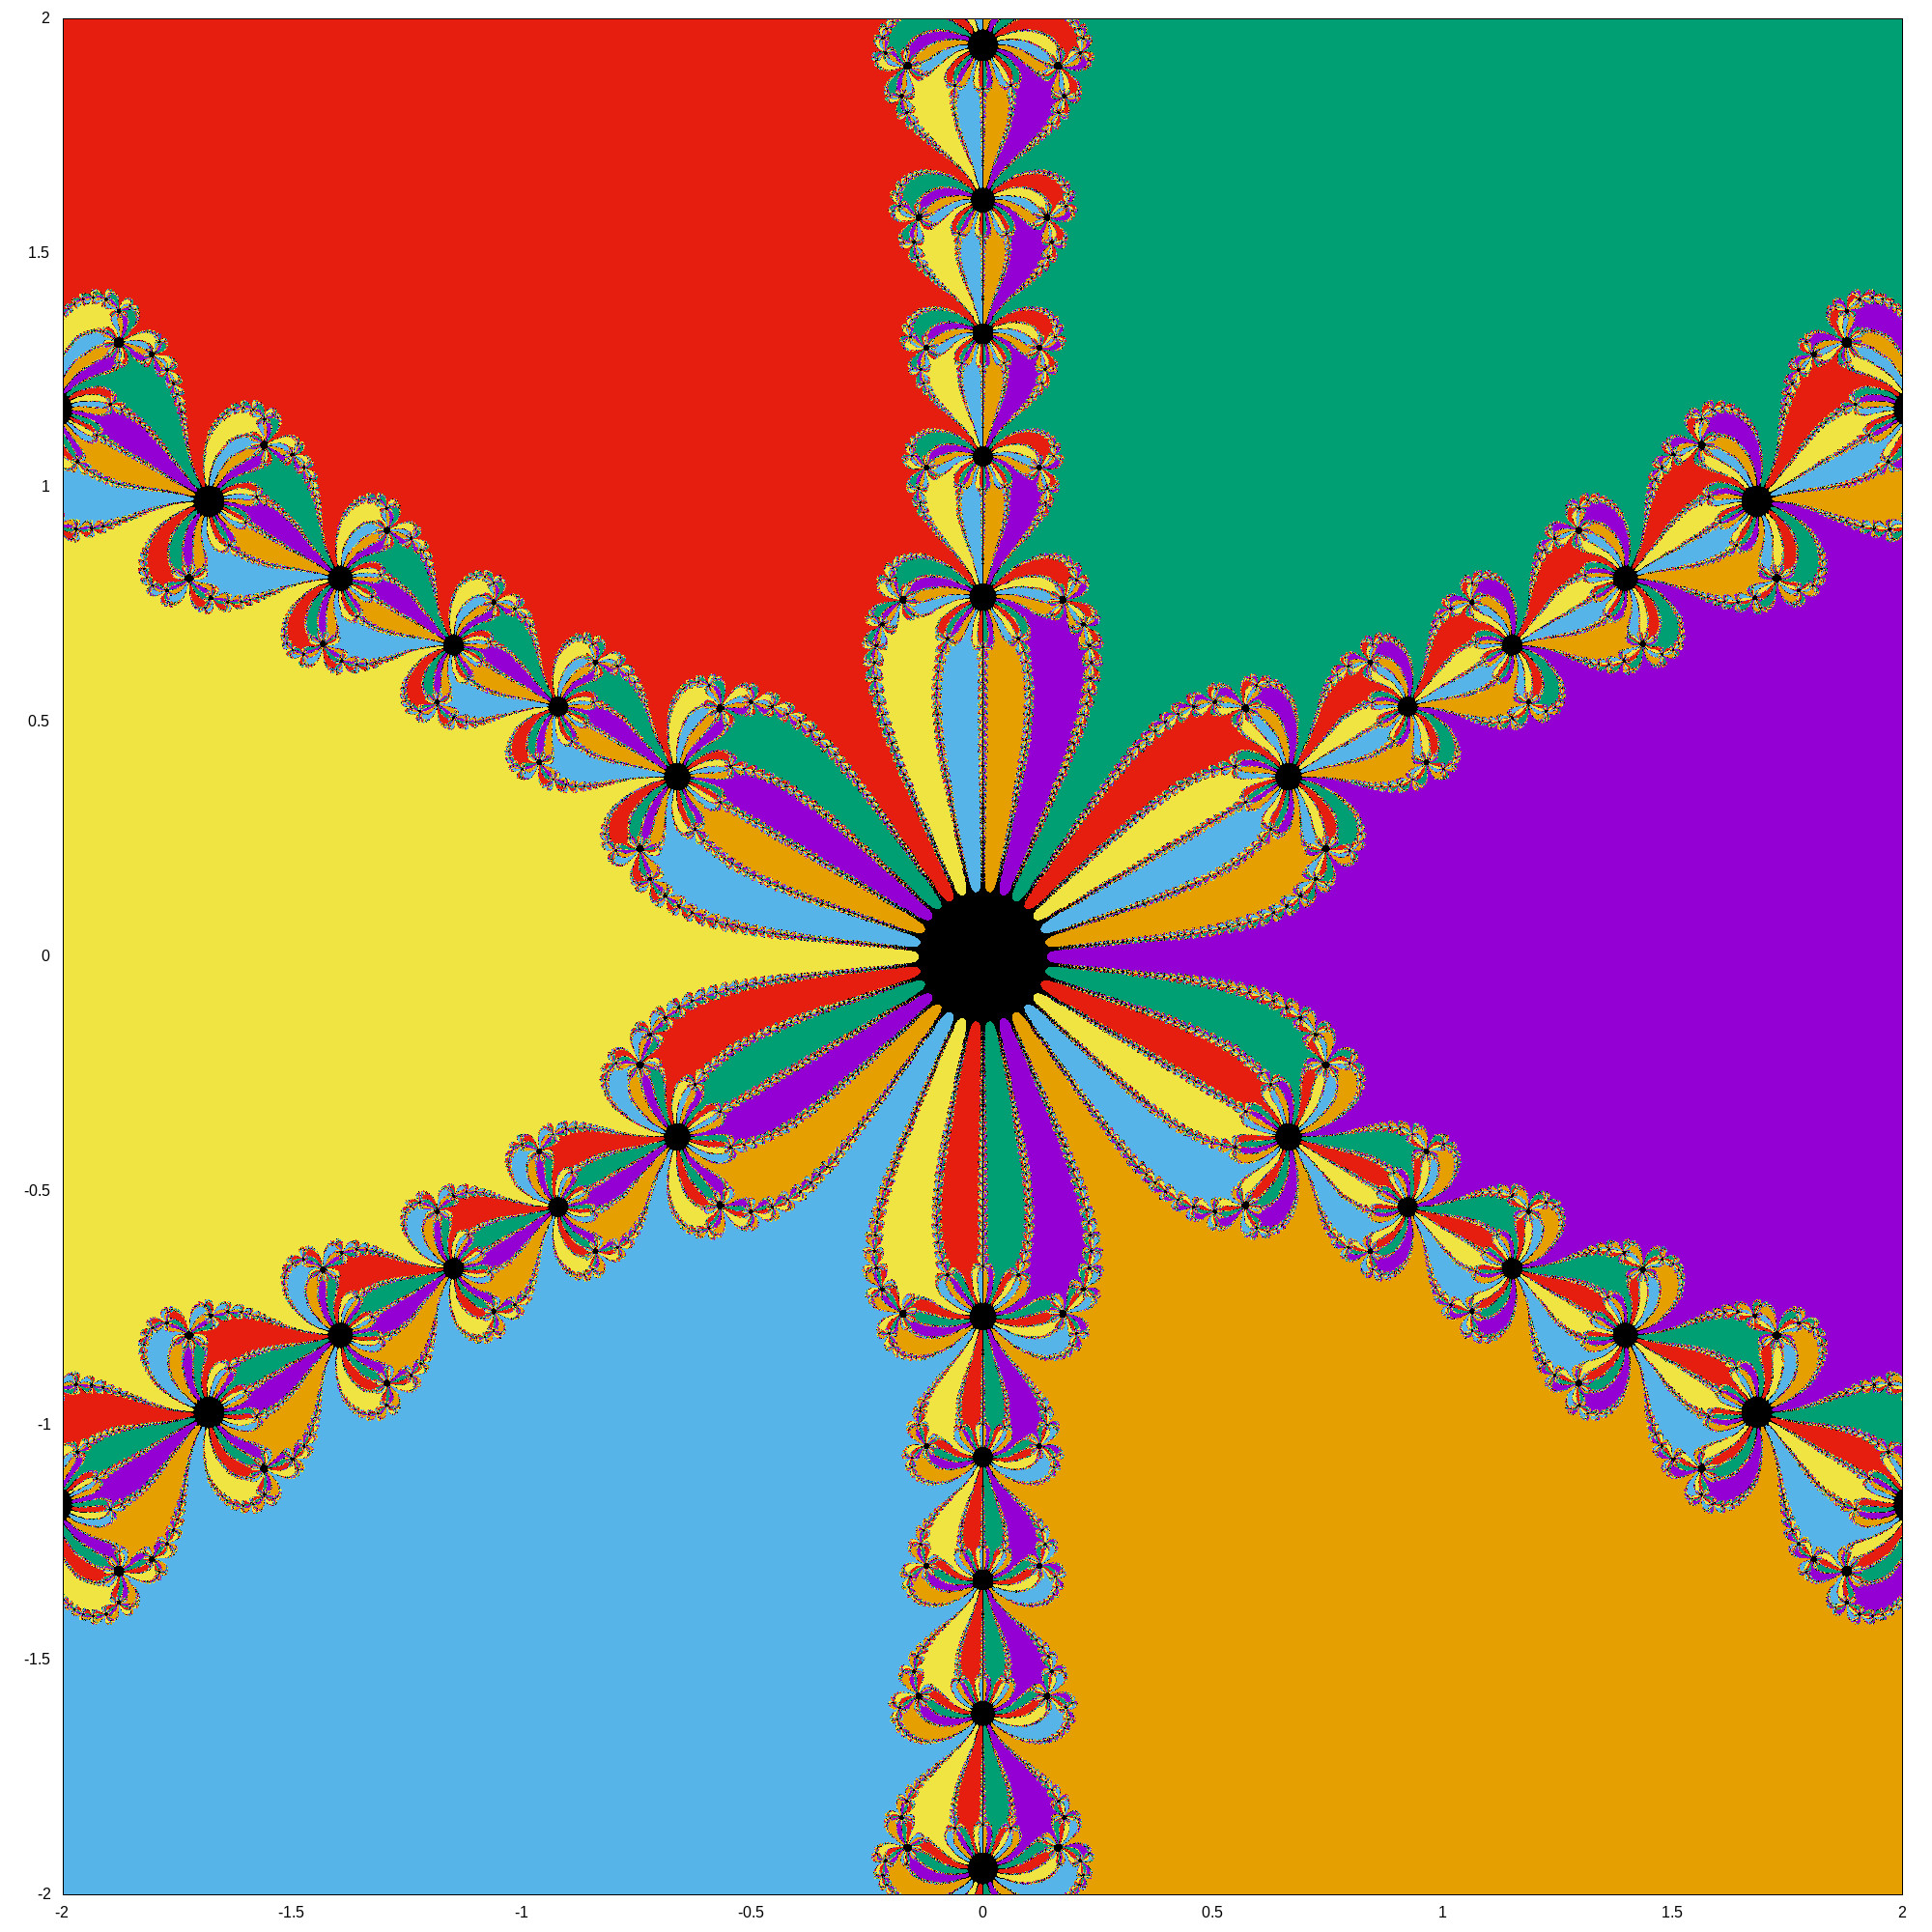
\includegraphics[width=\linewidth]{/home/giatro/Desktop/IME/3_Semestre/Laboratorio_de_Metodos_Numericos_MAC0210/EPs/1EP/f2.jpeg}
    \caption{$f_2(x)=x^6-1$}
\end{figure}

\begin{figure}
    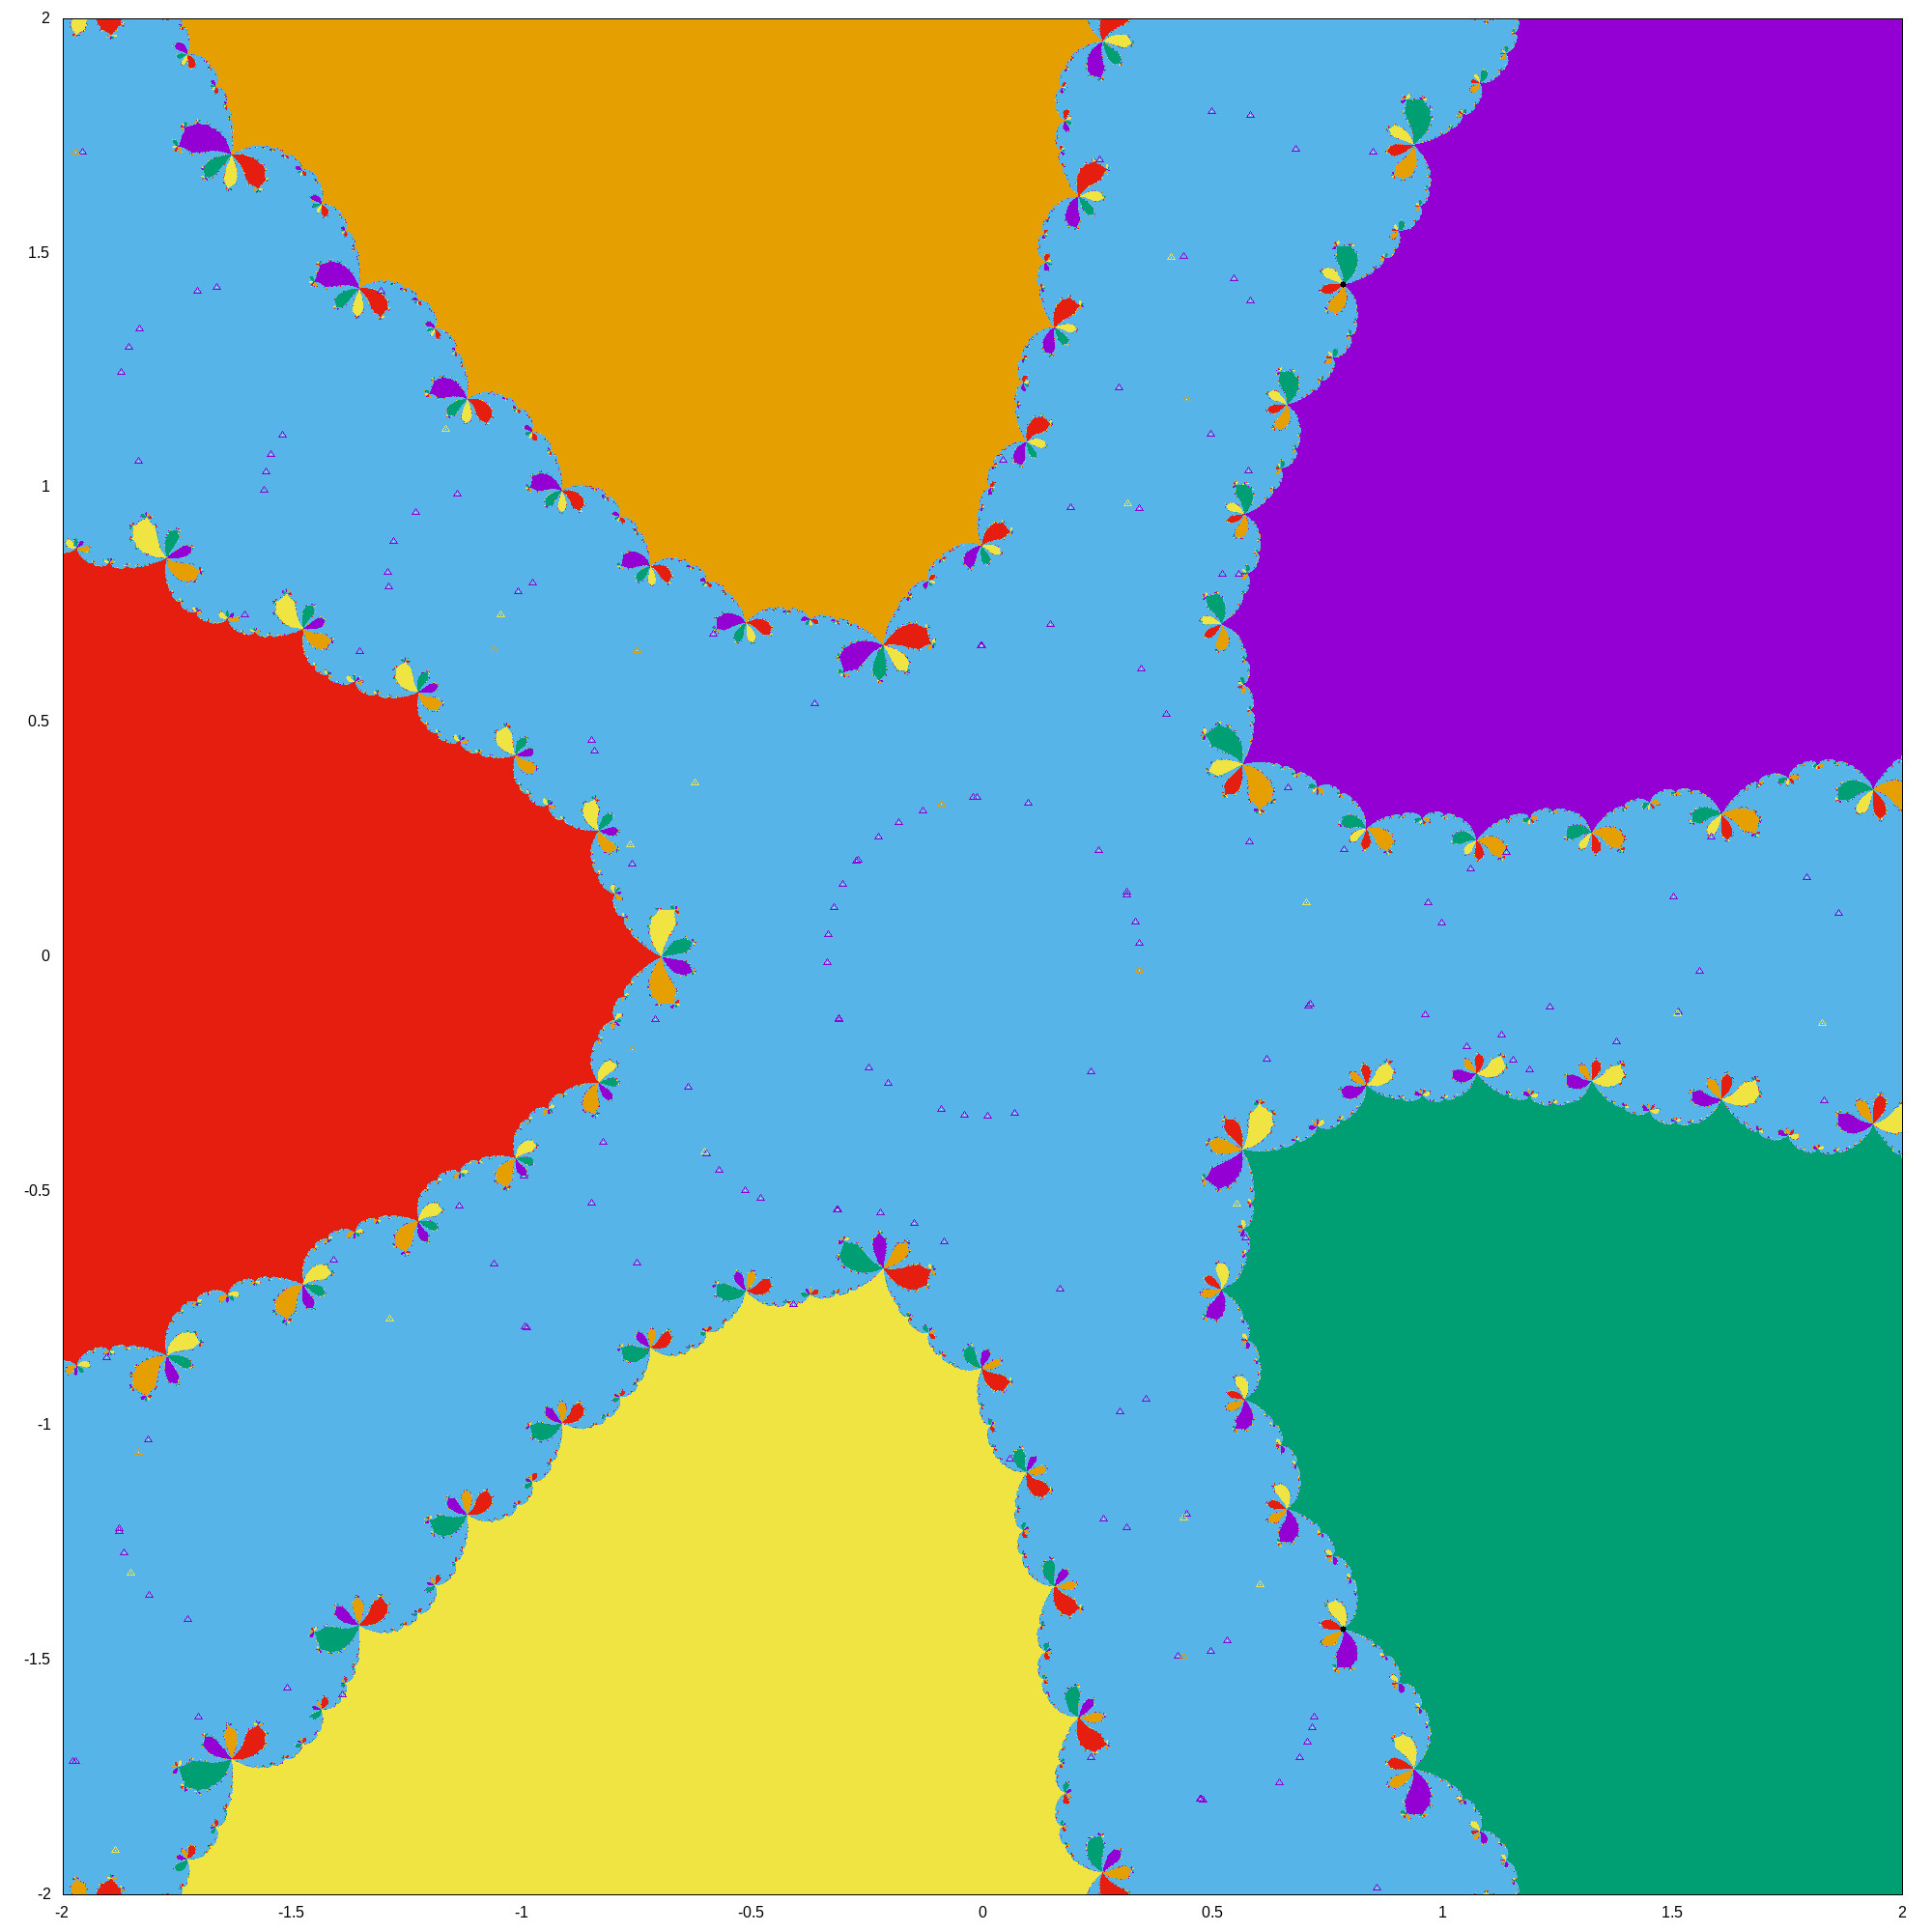
\includegraphics[width=\linewidth]{/home/giatro/Desktop/IME/3_Semestre/Laboratorio_de_Metodos_Numericos_MAC0210/EPs/1EP/f3.jpeg}
    \caption{$f_3(x)=x^6+x$}
\end{figure}

\begin{figure}
    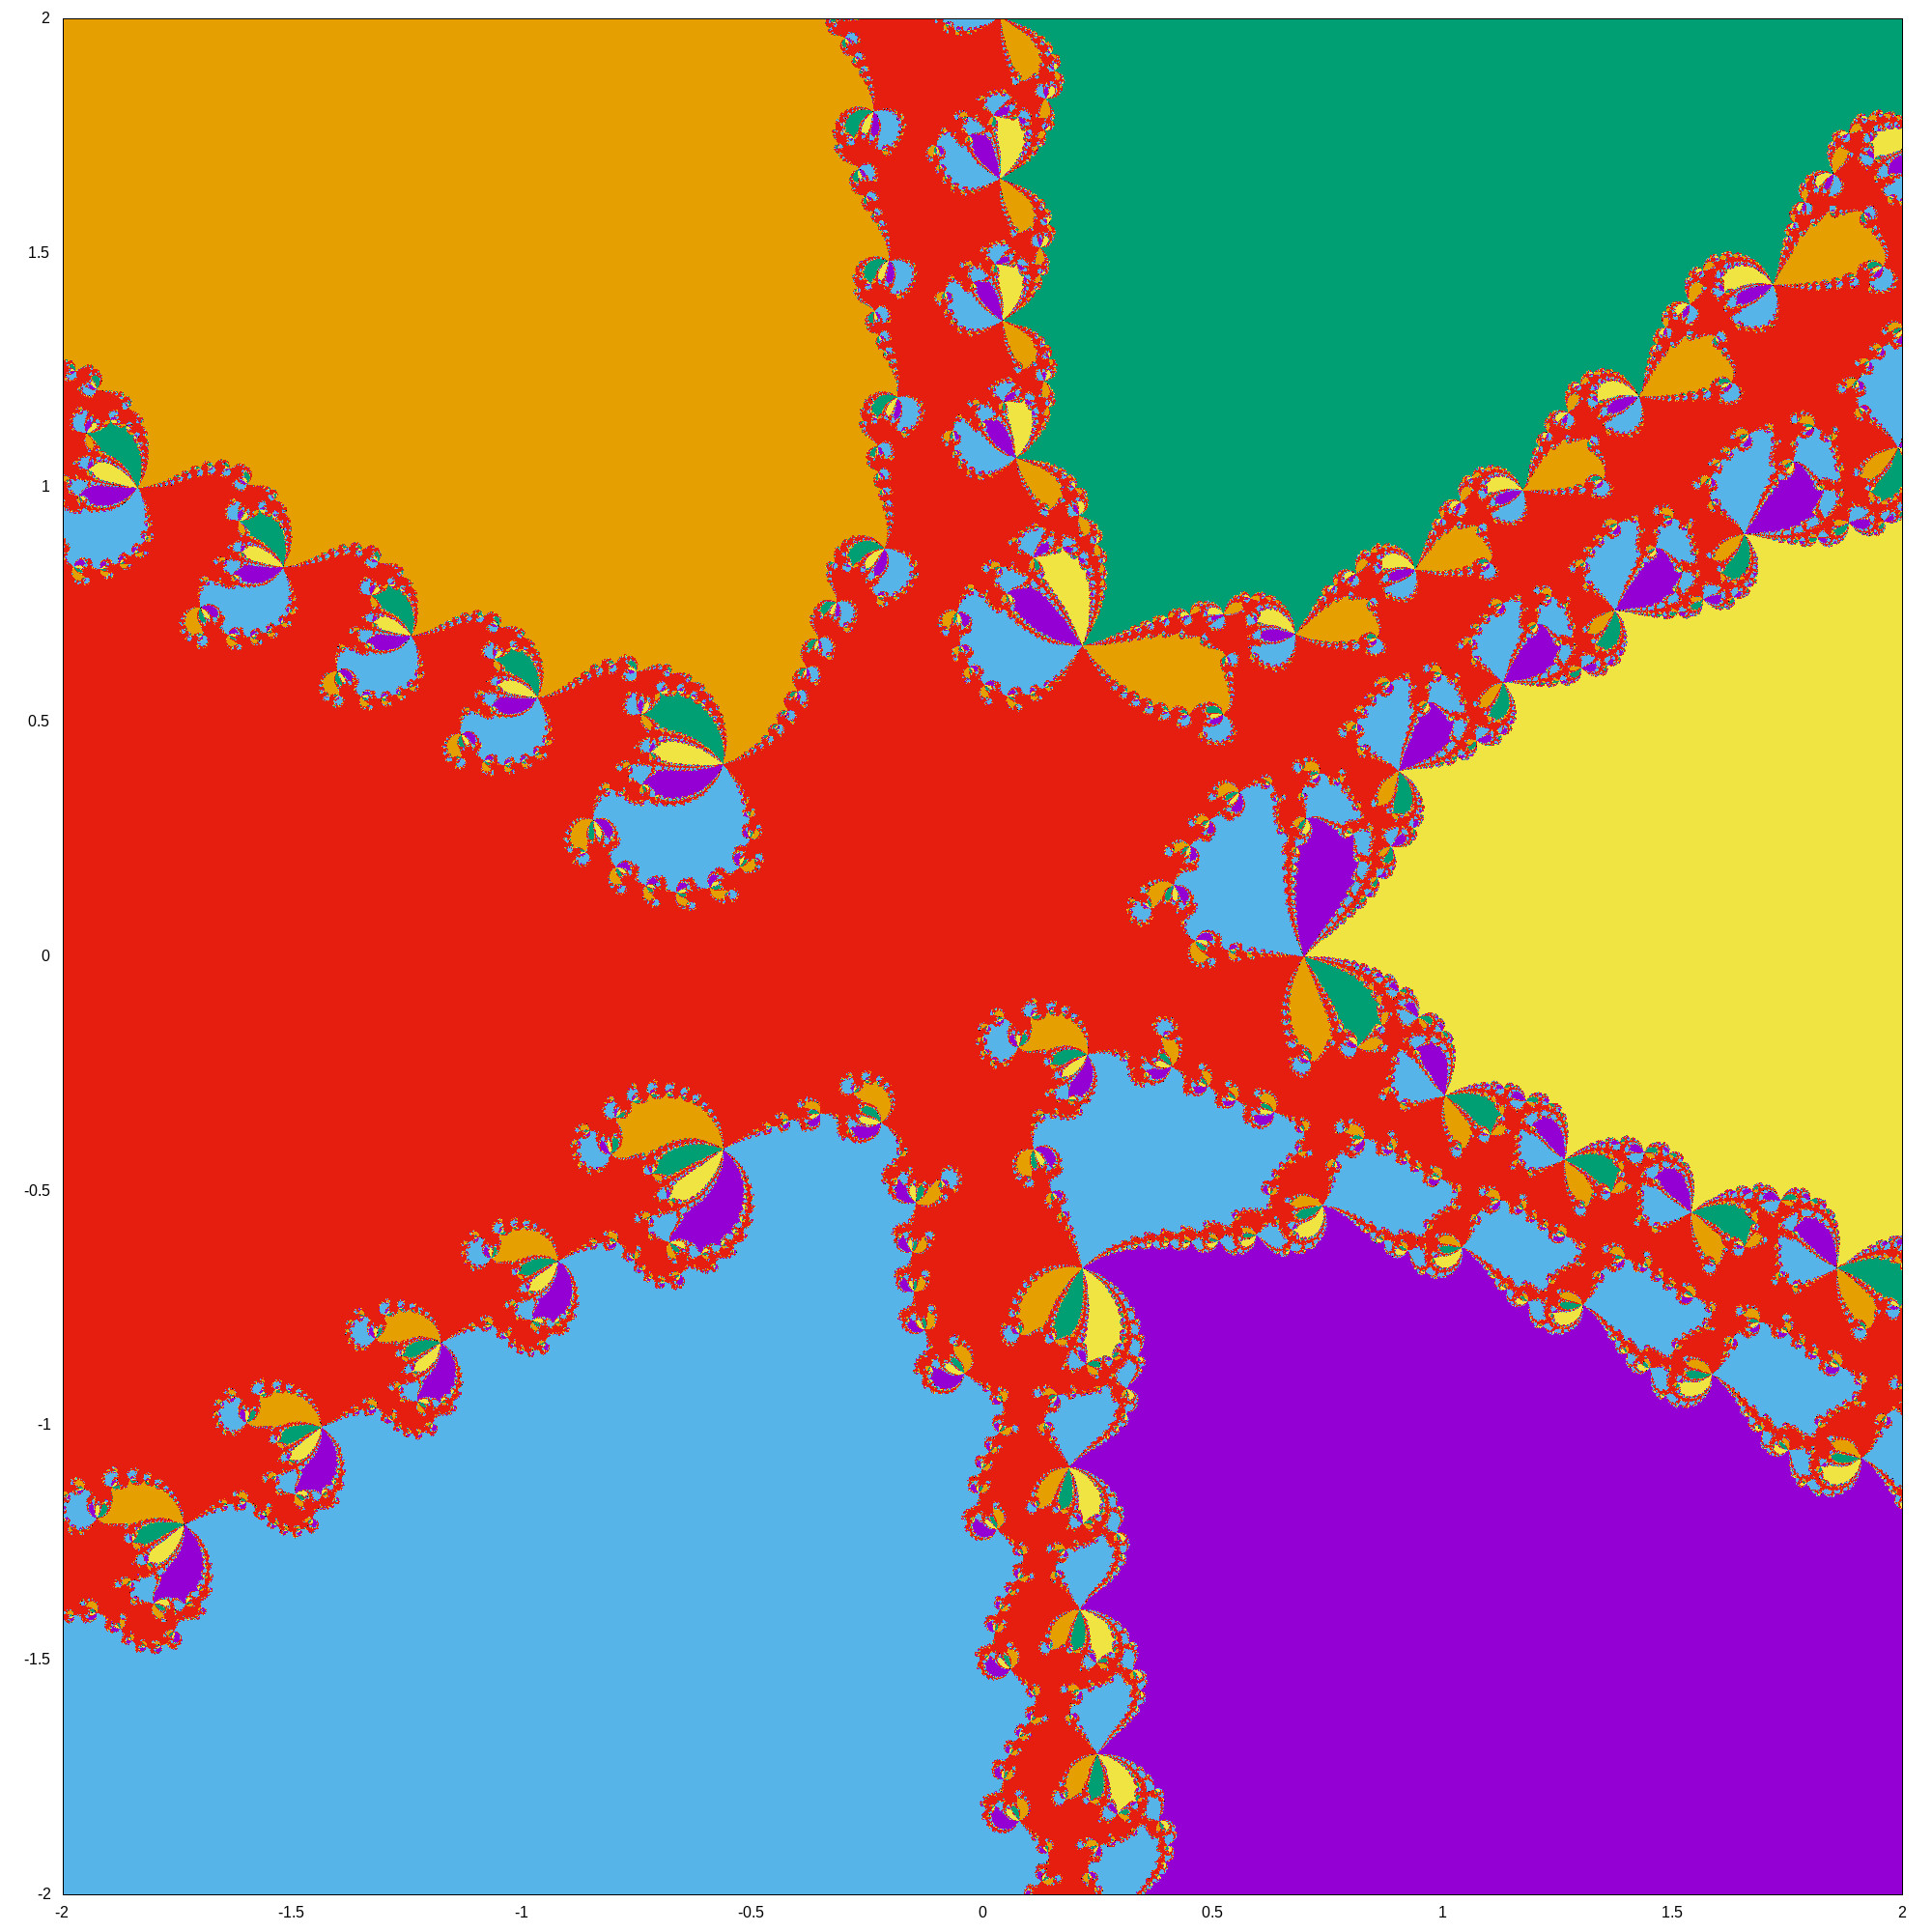
\includegraphics[width=\linewidth]{/home/giatro/Desktop/IME/3_Semestre/Laboratorio_de_Metodos_Numericos_MAC0210/EPs/1EP/f4.jpeg}
    \caption{$f_3(x)=x^6-x$}
\end{figure}

\begin{figure}
    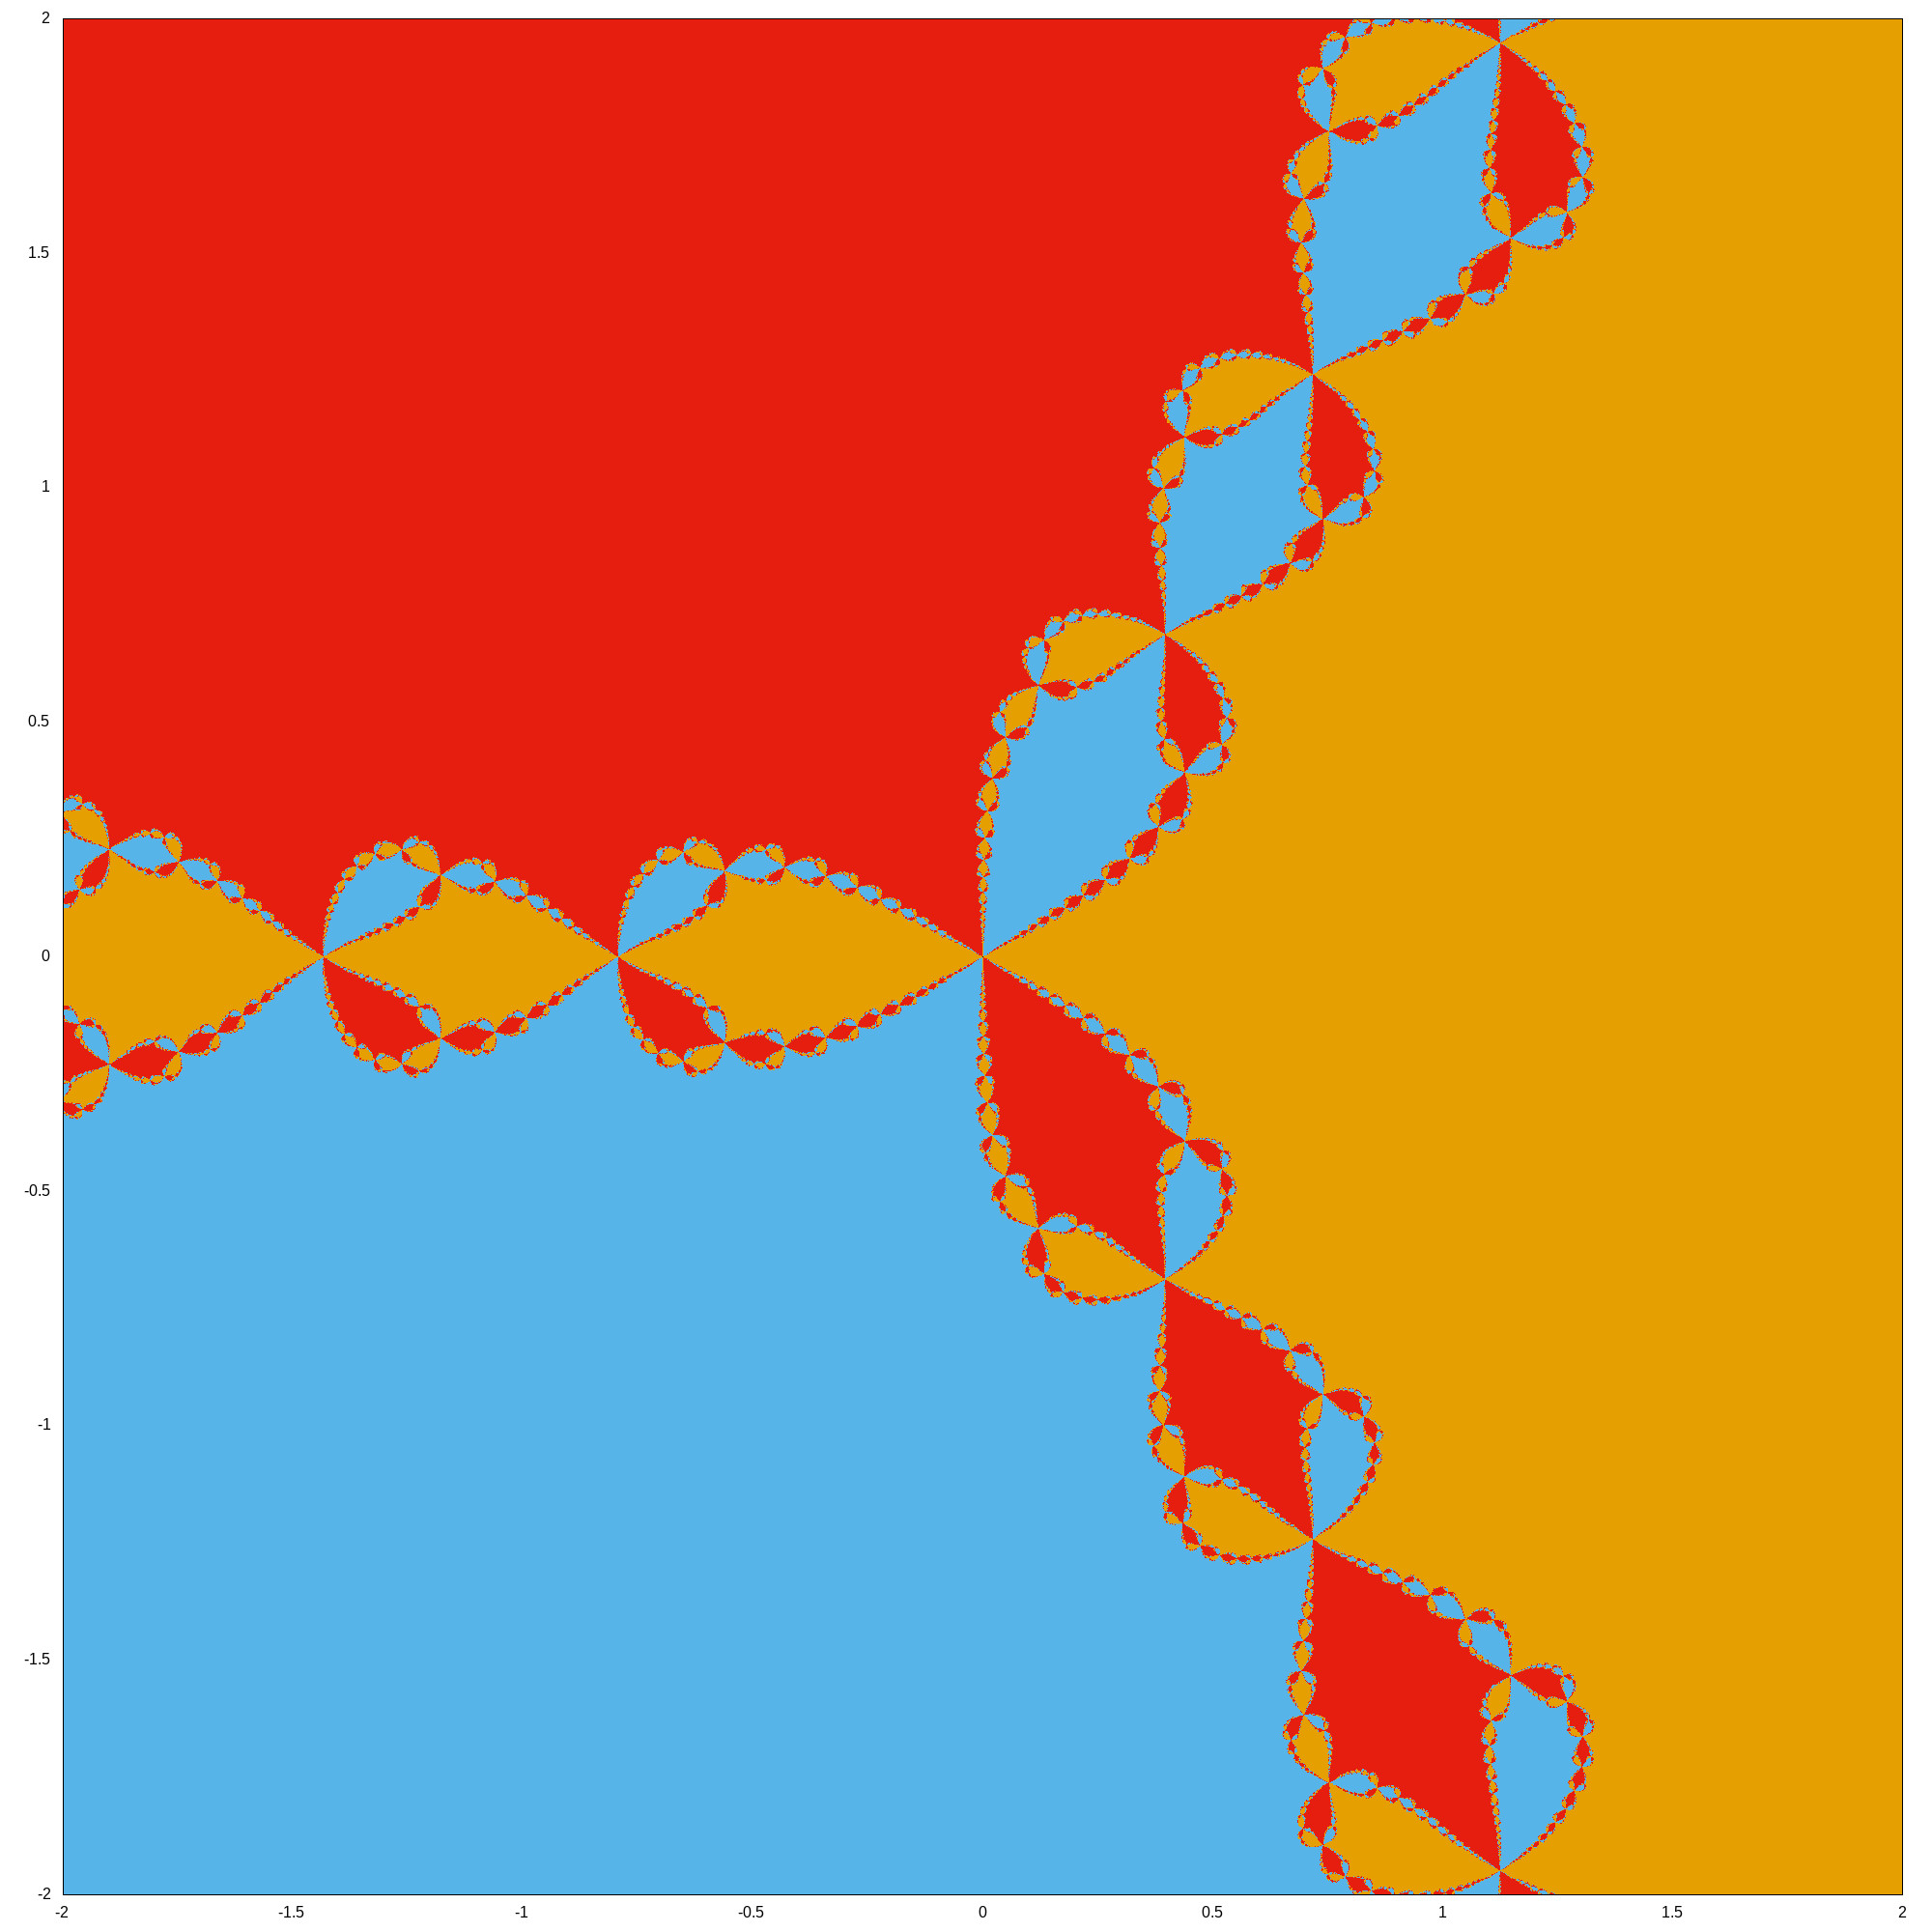
\includegraphics[width=\linewidth]{/home/giatro/Desktop/IME/3_Semestre/Laboratorio_de_Metodos_Numericos_MAC0210/EPs/1EP/f5.jpeg}
    \caption{$f_3(x)=x^3-1$}
\end{figure}

\end{document}